% Benchmark Evaluation Section

In order to verify and demonstrate the capabilities of the CircusTent benchmark suite, in this section we conduct an evaluation of a diverse set of platforms with respect to atomic memory operations.
We first introduce our test platforms and briefly describe pertinent details of their architecture in Section~\ref{subsec:platforms}.
We next detail our evaluation methodology in Section~\ref{subsec:methodology}.
Finally, we present and discuss the results of our evaluation in Section~\ref{subsec:results}.
\todo[inline]{@Brody - If we are short of space, this block of text can likely be omitted}
\todo[inline]{@John - The listed MEMSYS page limit is up to 16 pages, so we are likely good on space. It could still be removed though if it is extraneous.}

\subsection{Platforms}
\label{subsec:platforms}

We evaluate CircusTent across a total of fourteen distinct platforms that encompass device classes ranging from embedded systems to those used in petascale-class supercomputers.
These systems feature single and dual socket configurations utilizing processors from Intel, AMD, and ARM with varied instruction set architectures, clock frequencies, and core counts.
Similarly, the total memory capacity differs across platforms.
Table~\ref{tab:benchsys} provides an overview of our test platform specifications wherein each system is denoted by its processor model.
The size of the \texttt{VAL} array used during our evaluation, as well as the compiler used to build CircusTent, is also shown for each platform.

As the organization of each system's cache hierarchy is an important factor to its benchmark performance, some further detail in this regard is warranted.
Many of the processors featured in our test platforms adhere to a somewhat standard cache hierarchy design.
Each of these processors feature a three-level hierarchy wherein the L1 and L2 caches are private to each core and the L3 caches are shared between cores in a given socket.
Each L1 cache is subdivided into L1i and L1d caches for instructions and data, respectively.
For the sake of brevity, we detail only systems whose cache organization deviates from this norm, and how they do so, below.

\begin{itemize}
\item Cortex-A53 -
\newline
\item Cortex-A72 -
\newline
\item Core i7-4980HQ - In addition to a conventional 6 MiB L3 cache shared between cores, this processor also features a 128 MiB L4, or ``Crystal Well", cache that is shared between the CPU cores and the integrated GPU.
\newline
\item Xeon Phi 7250 - The 68 cores present in this processor are arranged in 34 tiles of 2 cores each.
Herein, cores coresident within a tile share a 1MiB L2 cache.
Although it does not incorporate a true shared last level cache, this processor features 16 GiB of MCDRAM that can be used as addressable memory, a shared cache across all cores, or in a hybrid configuration. 
For our evaluation, the MCDRAM is utilized in the cache configuration.
\end{itemize}

%\todo[inline]{John - Originally, I was going to list (at least cache) details for every platform here. However, I decided it might not look good to take up so much space and repeat a lot of info. I also elected to leave out the specific cache level sizes, associativity, and inclusivity. We can employ the original approach and/or add these details if preferable. - Brody}
%\todo[inline]{@Brody - I agree, lets leave out the underlying cache details for now.  If it becomes relevant in the evaluation section, we can outline the cache details for specific platforms.}
\todo[inline]{John - I was unsure of the precise Pi models for the cache info, but assumed they might also fit into this non-standard listing and added placeholders for now. - Brody}
\todo[inline]{@Brody - This is fixed in the table}
\todo[inline]{@John - Does either processor fit the "non-standard" criteria in the preceding paragraph and need to be included in the bulleted list?}

\begin{table*}
\caption{Benchmark System Configurations}
\label{tab:benchsys}
\begin{tabular}{ccccp{15mm}ccp{16mm}c}
\toprule
System&Clock Frequency&Cores / Socket&Total Sockets&LLC Size\newline~/ Socket&Total Memory&Array Size&Operating\newline System&Compiler\\
\midrule
Cortex-A53      & 1.40Ghz & 4  & 1 & 2MiB  & 512MiB & 256MiB  & Ubuntu\newline 18.04 4.15.0 & GCC 7.4.0\\
Cortex-A72      & 1.50Ghz & 4  & 1 & 1MiB   & 4GiB & 256MiB  & Debian\newline 10.1 4.19.75 & GCC 8.3.0\\
Ryzen V1605B    & 1.58Ghz & 4  & 1 & 4MiB    & 32GiB & 15GiB & Ubuntu\newline 19.04 5.2.10&GCC 8.3.0\\
Opteron 4130    & 2.60Ghz & 4  & 2 & 6MiB   & 64GiB & 15GiB & Centos7\newline 3.10.0&GCC 8.3.1\\
Core i5-3210M   & 2.50Ghz & 2  & 1 & 3MiB   & 4GiB & 256MiB & macOS\newline 10.13.6&clang 9.1.0\\
Core i7-3930K   & 3.20Ghz & 6  & 1 & 12MiB  & 64GiB & 15GiB & Linux Mint\newline 18.3 4.15.0&GCC 5.4.0\\
Core i7-4980HQ  & 2.80Ghz & 4  & 1 & 6MiB L3 +\newline 128MiB L4 & 16GiB & 15GiB & macOS\newline 10.15.3&GCC 9.2.0\\
Xeon Phi 7250   & 1.40Ghz & 68 & 1 & 16GiB \newline MCDRAM & 96GiB & 15GiB & SLES\newline 4.12.14&GCC 8.3.0\\
Xeon E5620      & 2.40Ghz & 4  & 2 & 12MiB & 48GiB & 15GiB & Ubuntu\newline 16.04 4.4.0&GCC 5.4.0\\
Xeon X5650      & 2.67Ghz & 6  & 2 & 12MiB & 64GiB & 15GiB & Ubuntu\newline 18.04 4.15.0&GCC 7.5.0\\
Xeon E5-2620 v3 & 2.40Ghz & 6  & 1 & 15MiB & 64GiB & 15GiB & Ubuntu\newline 16.04 4.4.0&GCC 5.4.0\\
Xeon E5-2670 v2 & 2.50Ghz & 10 & 2 & 25MiB & 64GiB & 15GiB & Centos7\newline 3.10.0&GCC 7.3.0\\
Xeon E5-2695 v4 & 2.10Ghz & 18 & 2 & 45MiB & 192GiB & 15GiB & Centos7\newline 3.10.0&GCC 7.3.0\\
Xeon E5-2698 v3 & 2.30Ghz & 16 & 2 & 40MiB & 128GiB & 15GiB & SLES\newline 4.12.14&GCC 8.3.0\\
\bottomrule
\end{tabular}
\end{table*}

%\todo[inline]{John - I pulled the array sizes from the scripts files and the processor specs from the web. You can double check that everything looks correct if you want. From the OS info you sent on the Ryzen system, the cache size seems to correspond to the L2, so I am assuming the shared L3 is also present underneath. - Brody}
%\todo[inline]{@Brody - This is fixed}

\subsection{Methodology}
\label{subsec:methodology}

Consistent with previous studies \cite{villa2008barriers}\cite{david2013sync}\cite{schweizer2015evaluating}\cite{hoseini2019modeling}, we perform our initial evaluation of the CircusTent suite in the context of a physically shared memory environment.
In order to do so, we execute each of the CircusTent benchmark kernels, detailed in Section~\ref{subsec:algorithms}, on the test platforms introduced above using our OpenMP backend.
For each kernel, we conduct trials using implementations based on both the atomic \textit{Add} and \textit{Compare-and-Swap} primitives.
A uniform stride size of $N=9$ is utilized for each trial of the StrideN kernel.

We collect performance results for each platform.
In order to eliminate any performance volatility associated with simultaneous multithreading (SMT), we vary the thread count during our trials from a single thread, up to one thread per physical core, for each platform.
Similarly, 64-bit operands are used throughout the evaluation to prevent any inconsistencies.
Moreover, to better simulate real-world behavior, we allow the operating system and programming model to perform the mapping of threads to processor cores.

Where feasible, a uniform size of approximately 15 GiB is utilized for the \texttt{VAL} array on each platform.
For the Cortex A-53, Cortex A-72, and Core i5-3210M systems, wherein physical memory limitations make this configuration impractical, a 256 MiB \texttt{VAL} array is utilized instead.
In order to generate sufficient runtime such that observable patterns of behavior emerge, twenty million iterations of each kernel loop are run during every benchmark trial.
We utilize our normalized \textit{GAMs} metric, as introduced in Section~\ref{subsec:normalizingtheresults}, throughout our evaluation to measure and compare the performance of our diverse set of test platforms.

%\todo[inline]{John - Do you think it is alright to approximate the array size to 15GB? The exact size of 16488974000 bytes (approx. 15.36 GB) just looks a bit odd and seems arbitrary. - Brody}
%\todo[inline]{@Brody - Yes, this should be fine.  I difference between 15.36 and 16 GB will not affect these results}

\subsection{Results}
\label{subsec:results}

\begin{figure}[!t]
\centering
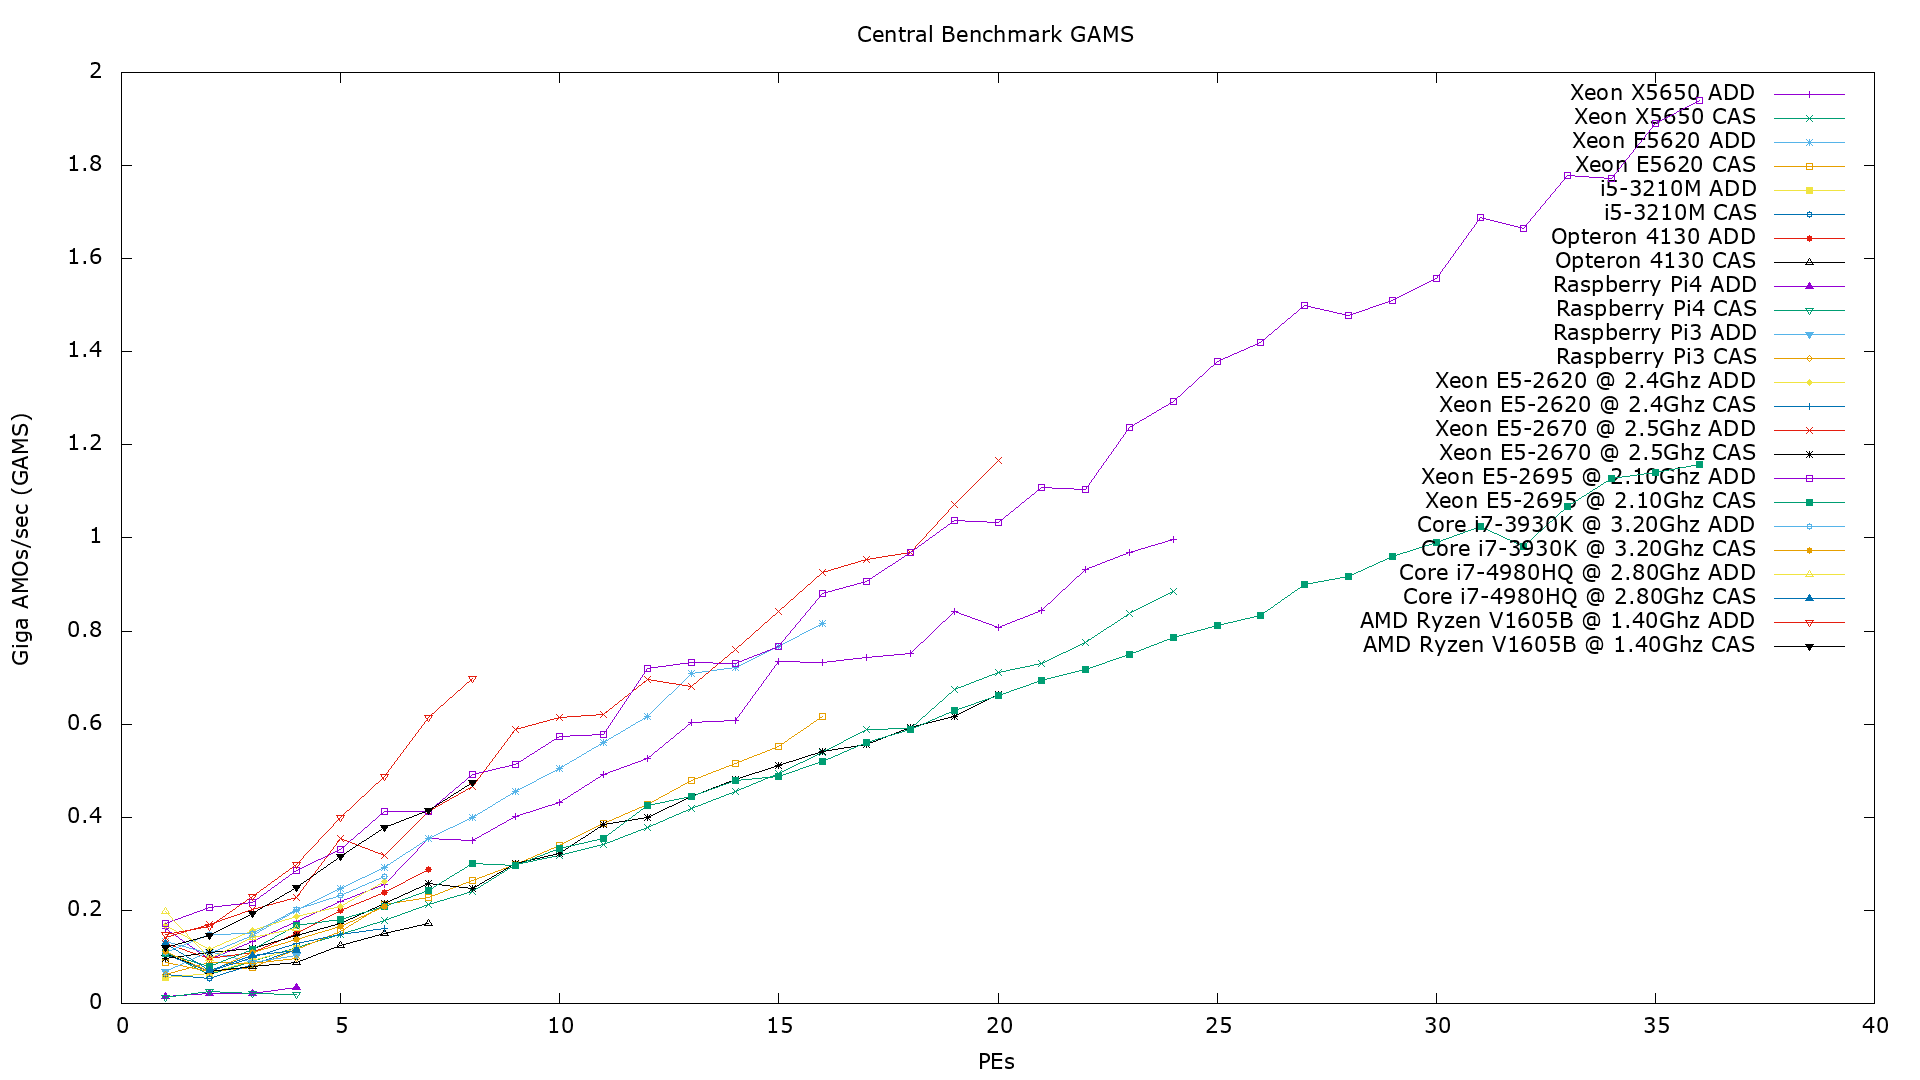
\includegraphics[width=3.5in]{figures/CENTRAL_GAMS.png}
\caption{Central Benchmark GAMS}
\label{fig:central_gams}
\end{figure}

\begin{figure}[!t]
\centering
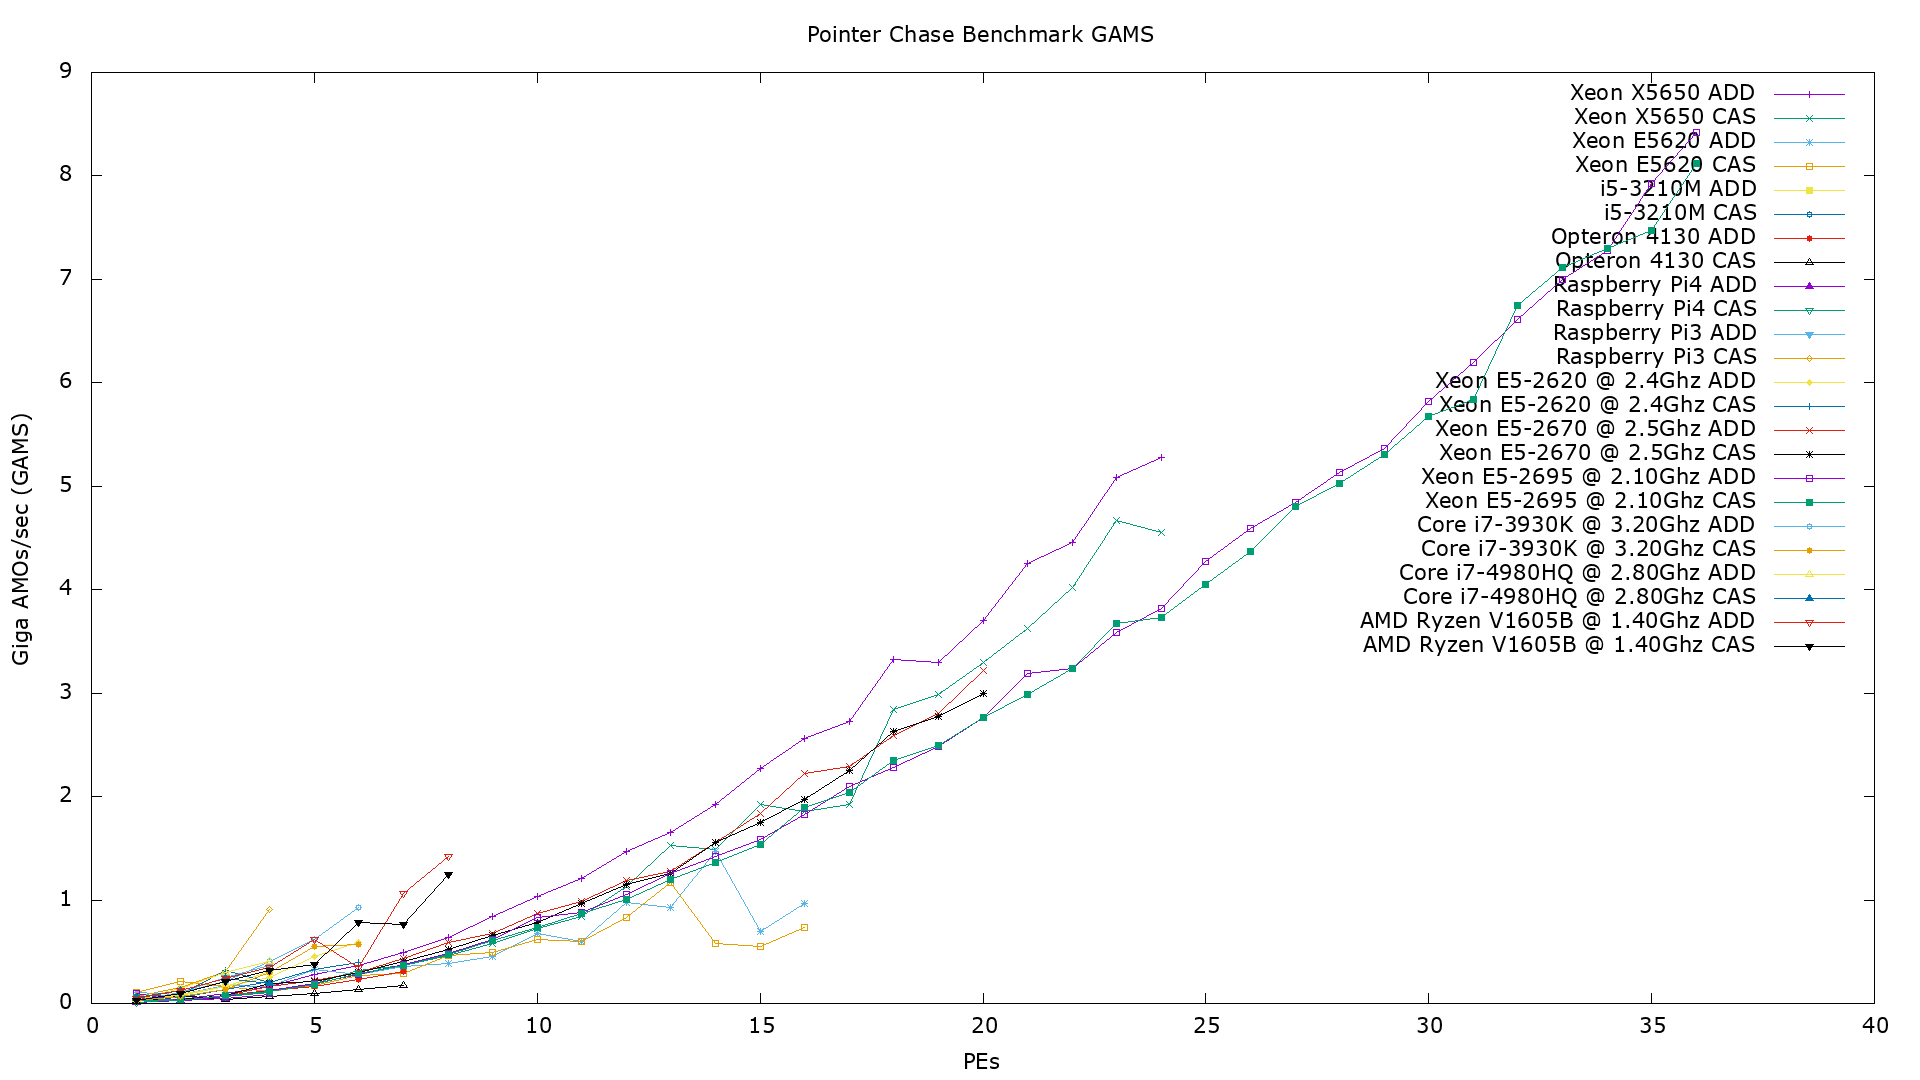
\includegraphics[width=3.5in]{figures/PTRCHASE_GAMS.png}
\caption{Pointer Chase Benchmark GAMS}
\label{fig:ptrchase_gams}
\end{figure}

\begin{figure}[!t]
\centering
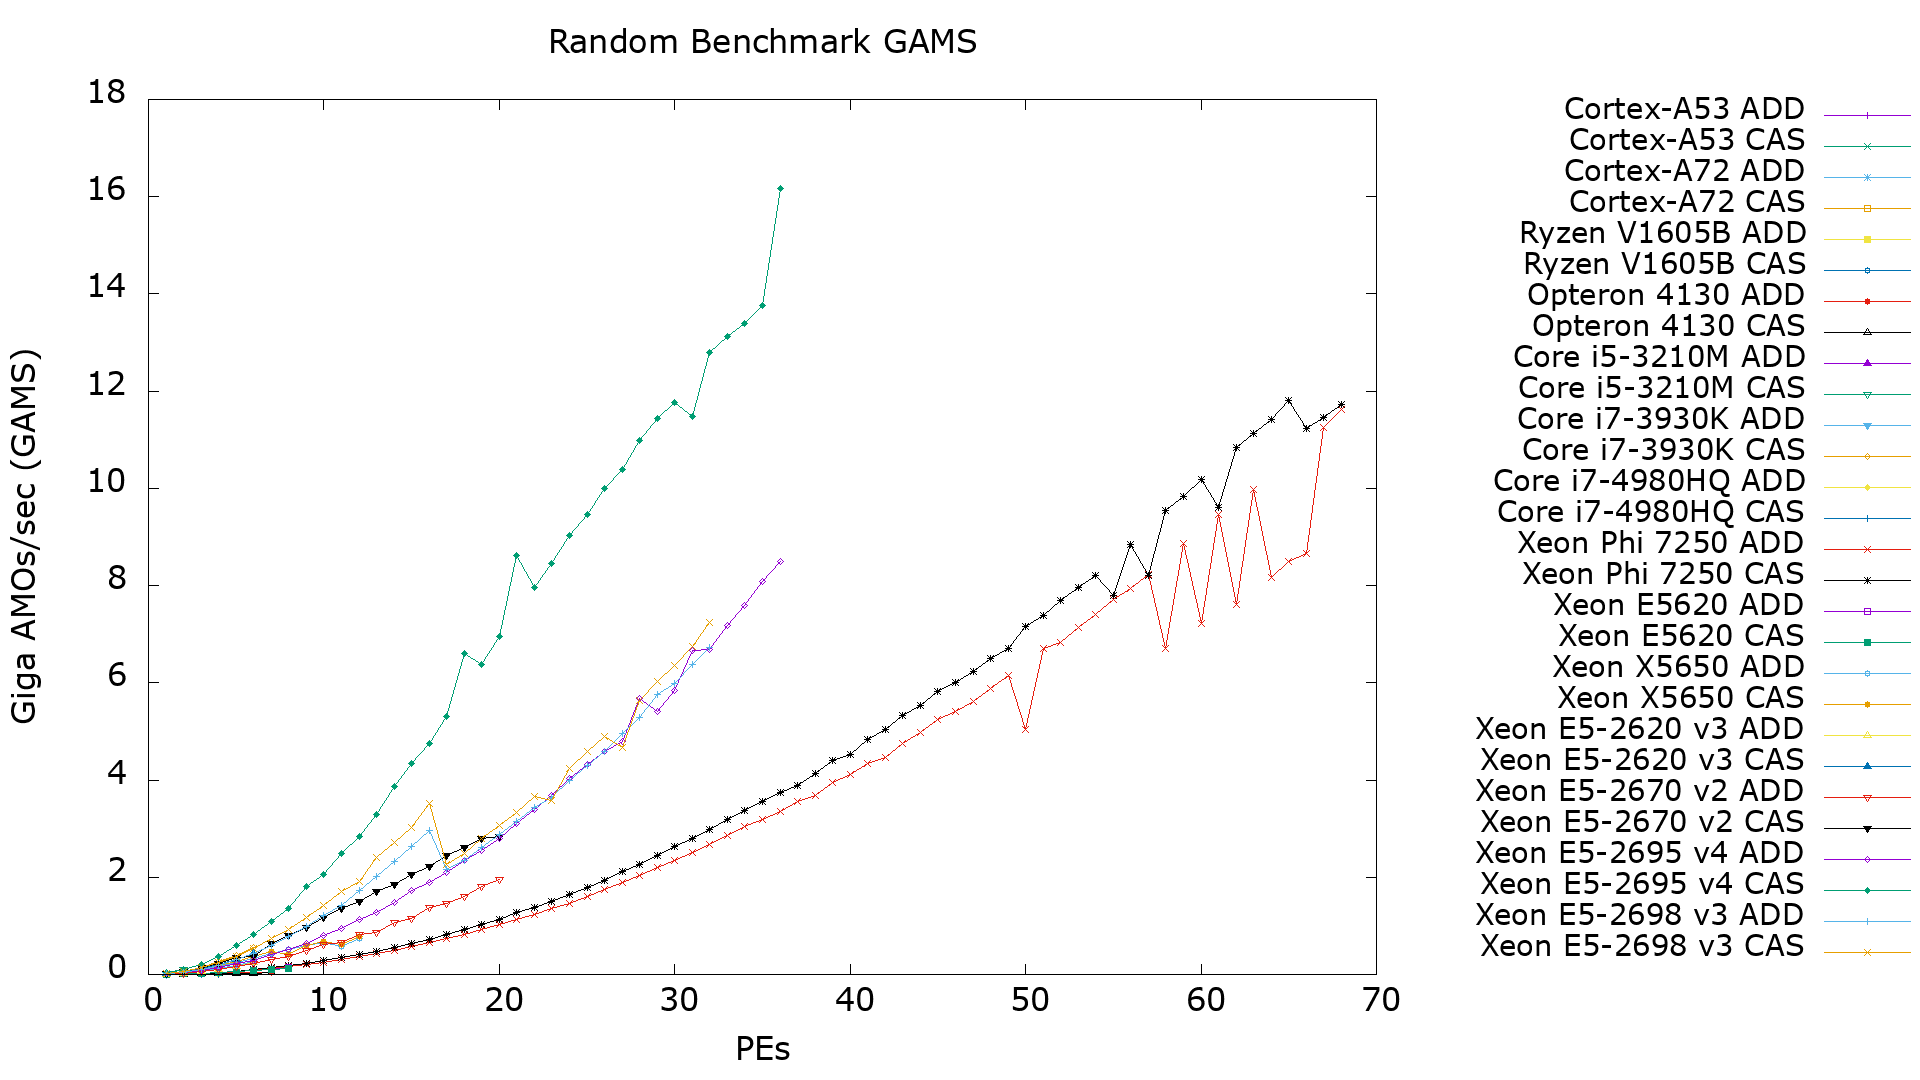
\includegraphics[width=3.5in]{figures/RAND_GAMS.png}
\caption{Random Benchmark GAMS}
\label{fig:rand_gams}
\end{figure}

\begin{figure}[!t]
\centering
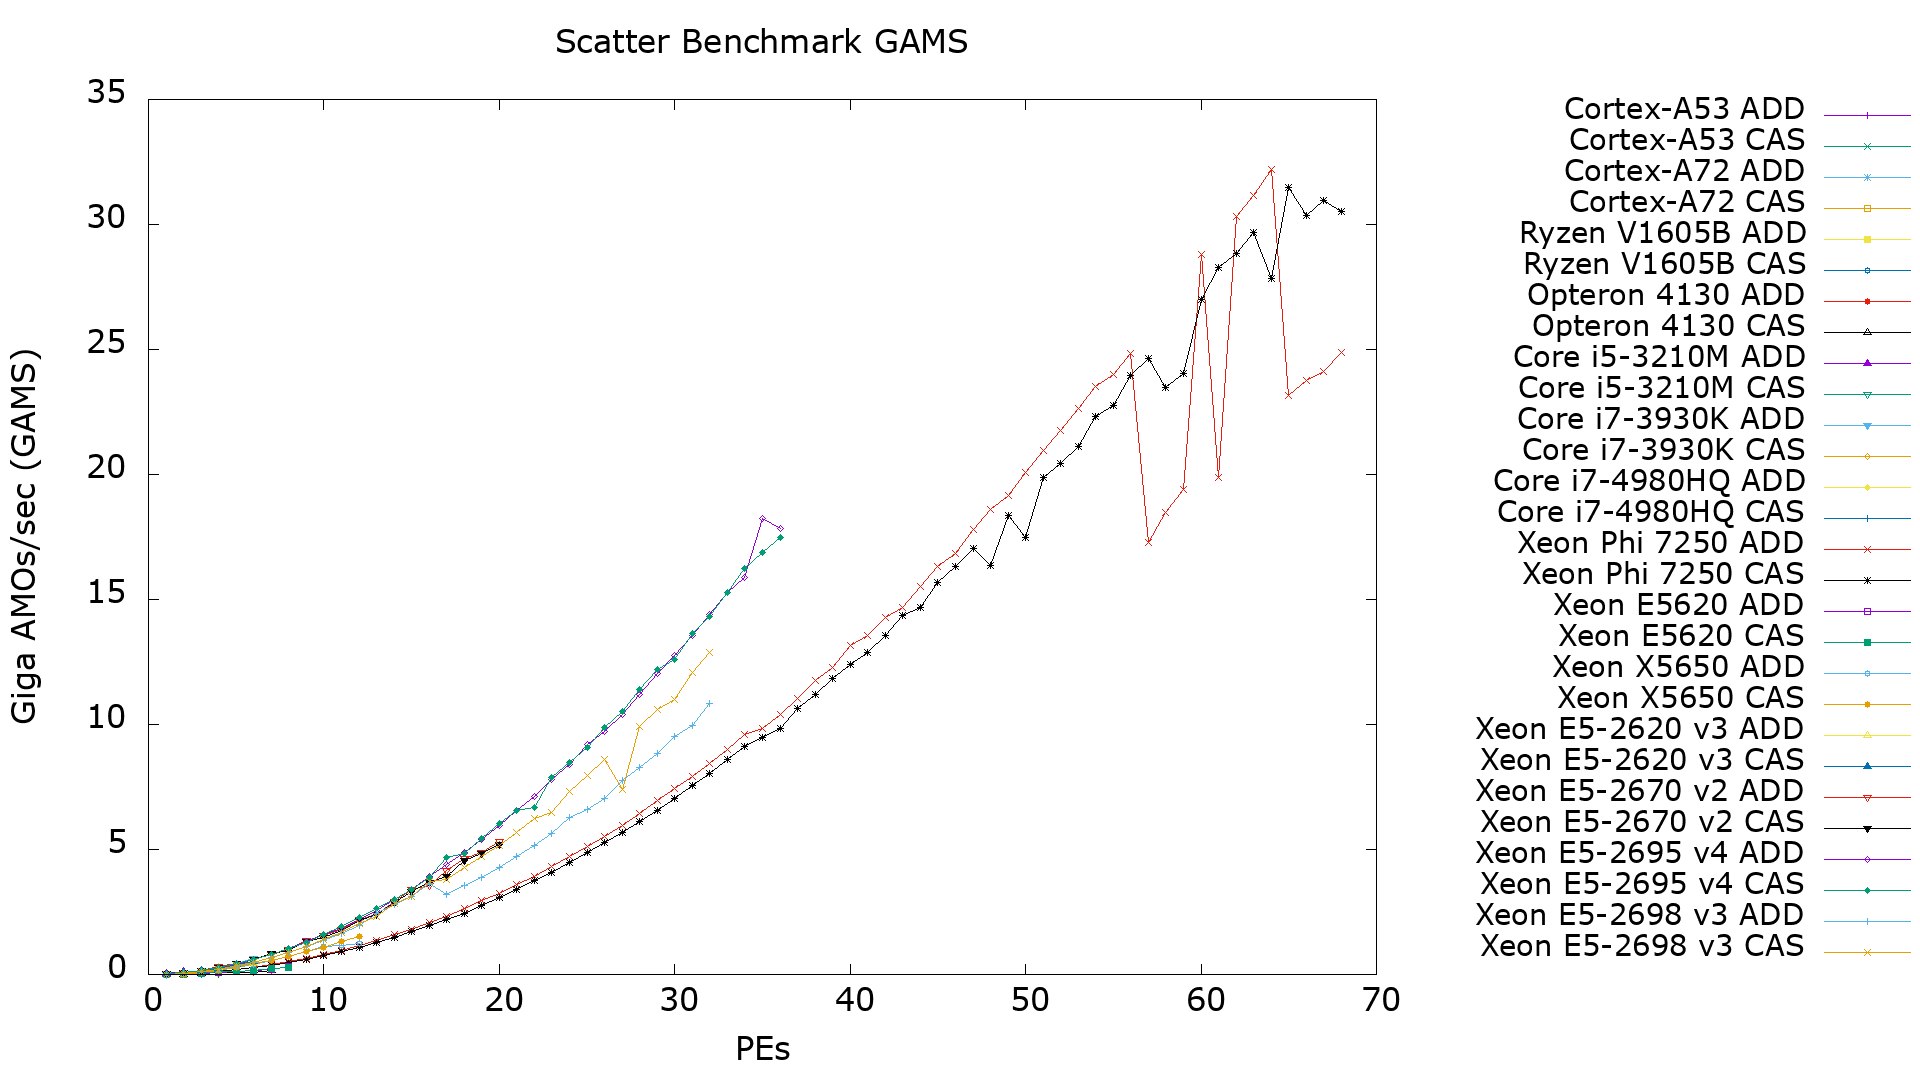
\includegraphics[width=3.5in]{figures/SCATTER_GAMS.png}
\caption{Scatter Benchmark GAMS}
\label{fig:scatter_gams}
\end{figure}

\begin{figure}[!t]
\centering
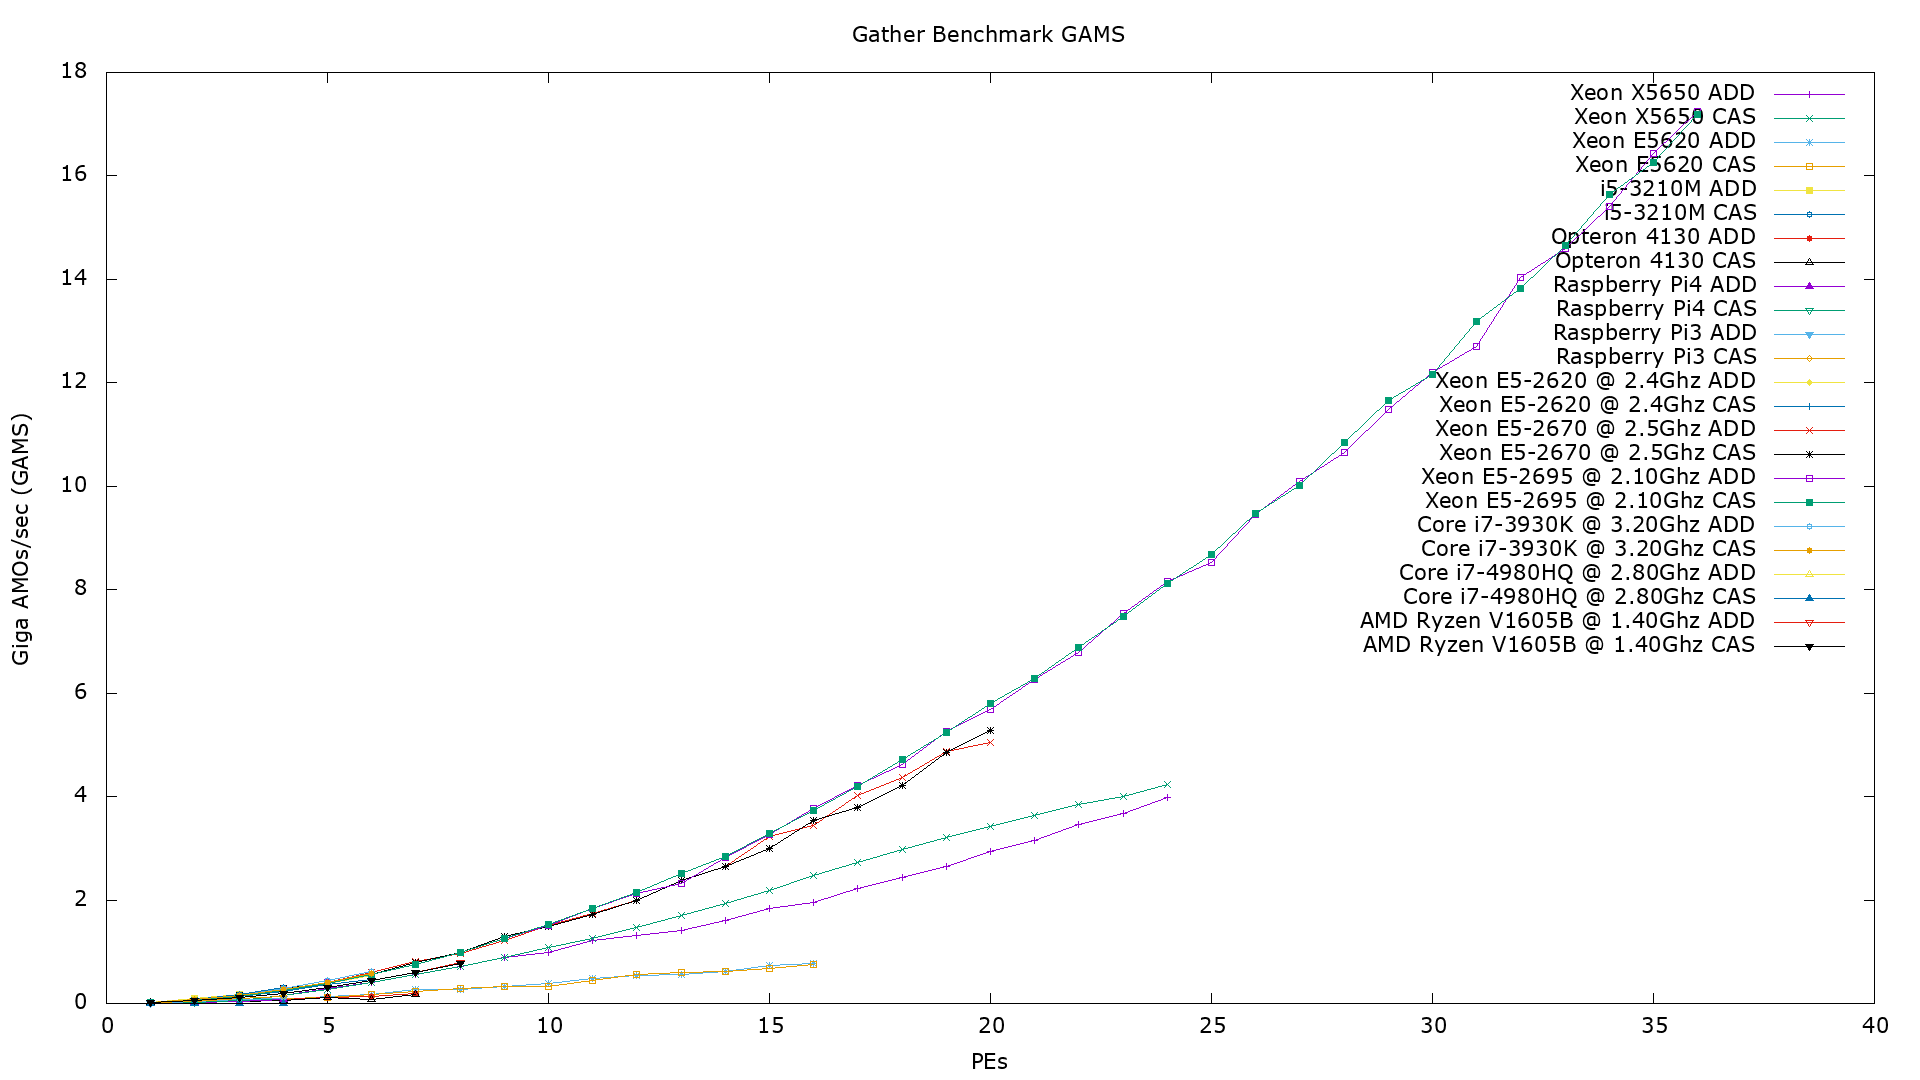
\includegraphics[width=3.5in]{figures/GATHER_GAMS.png}
\caption{Gather Benchmark GAMS}
\label{fig:gather_gams}
\end{figure}

\begin{figure}[!t]
\centering
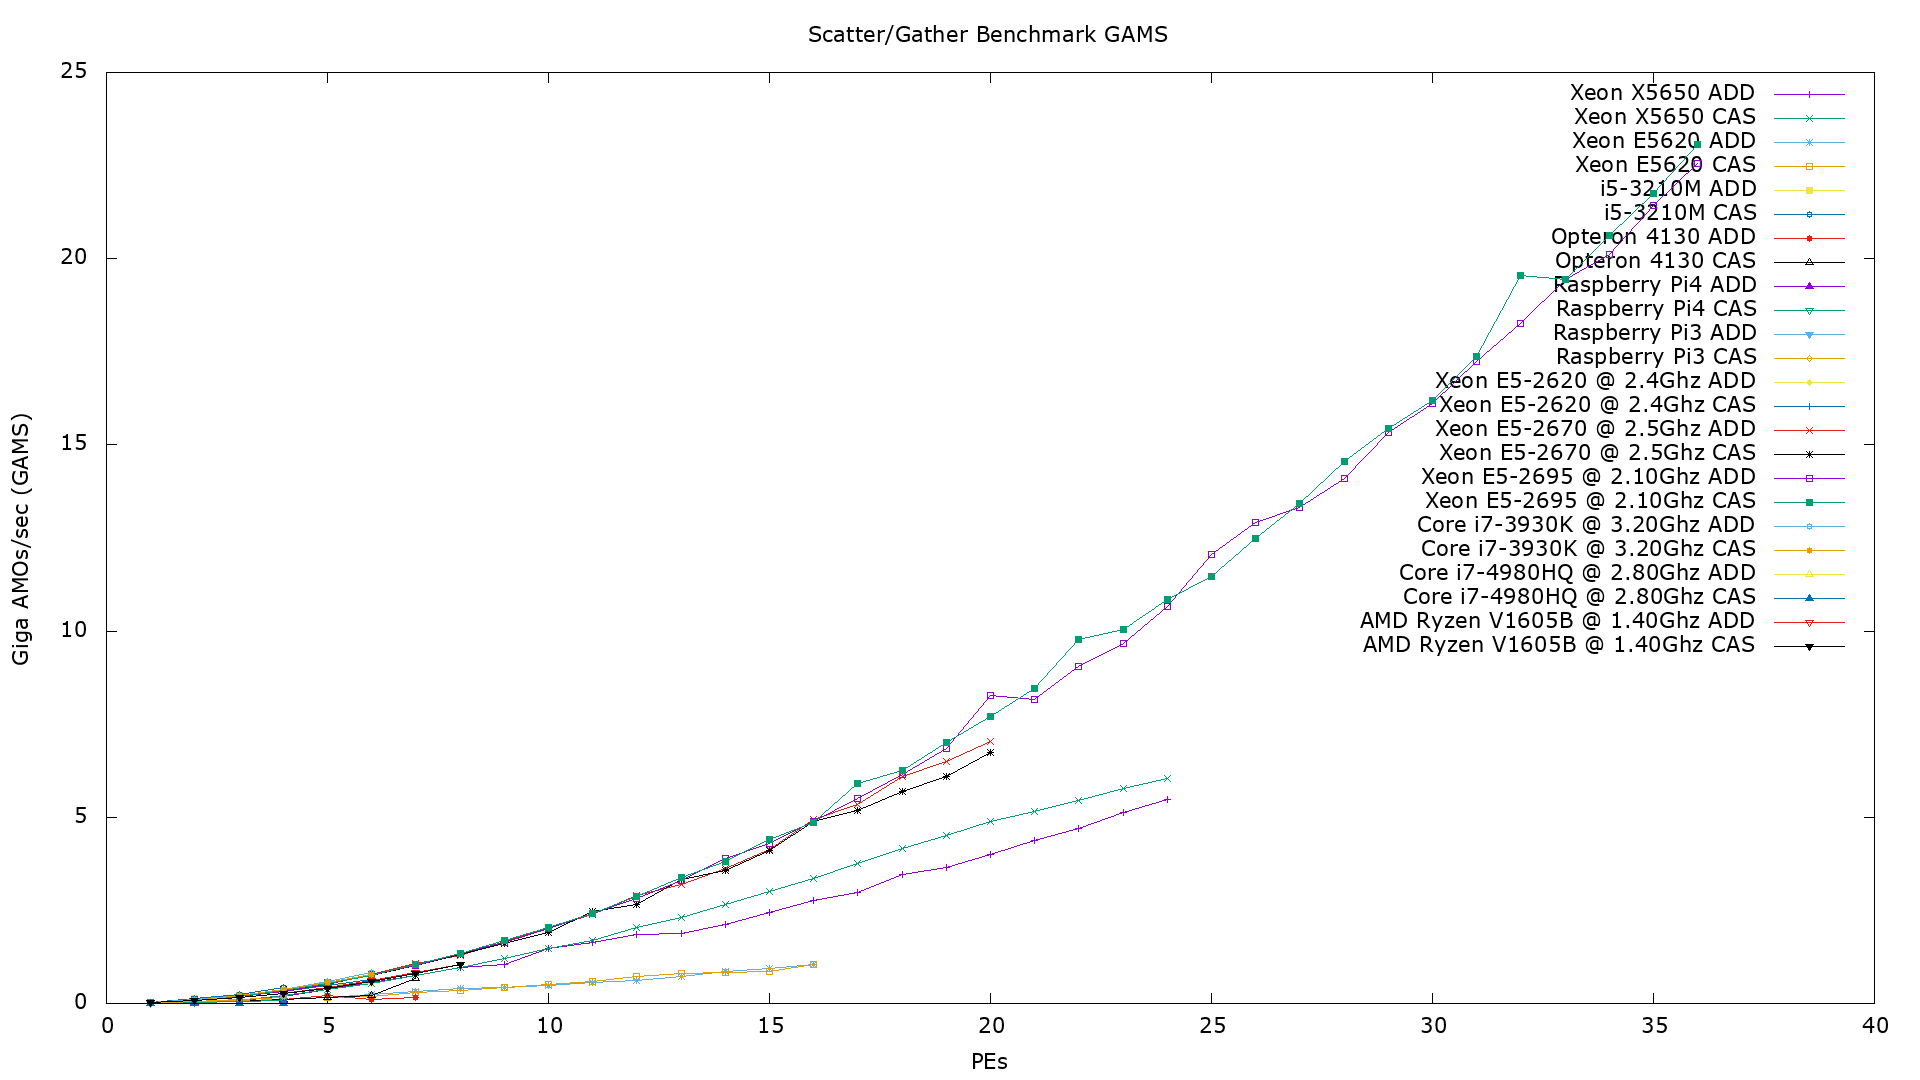
\includegraphics[width=3.5in]{figures/SG_GAMS.png}
\caption{Scatter/Gather Benchmark GAMS}
\label{fig:sg_gams}
\end{figure}

\begin{figure}[!t]
\centering
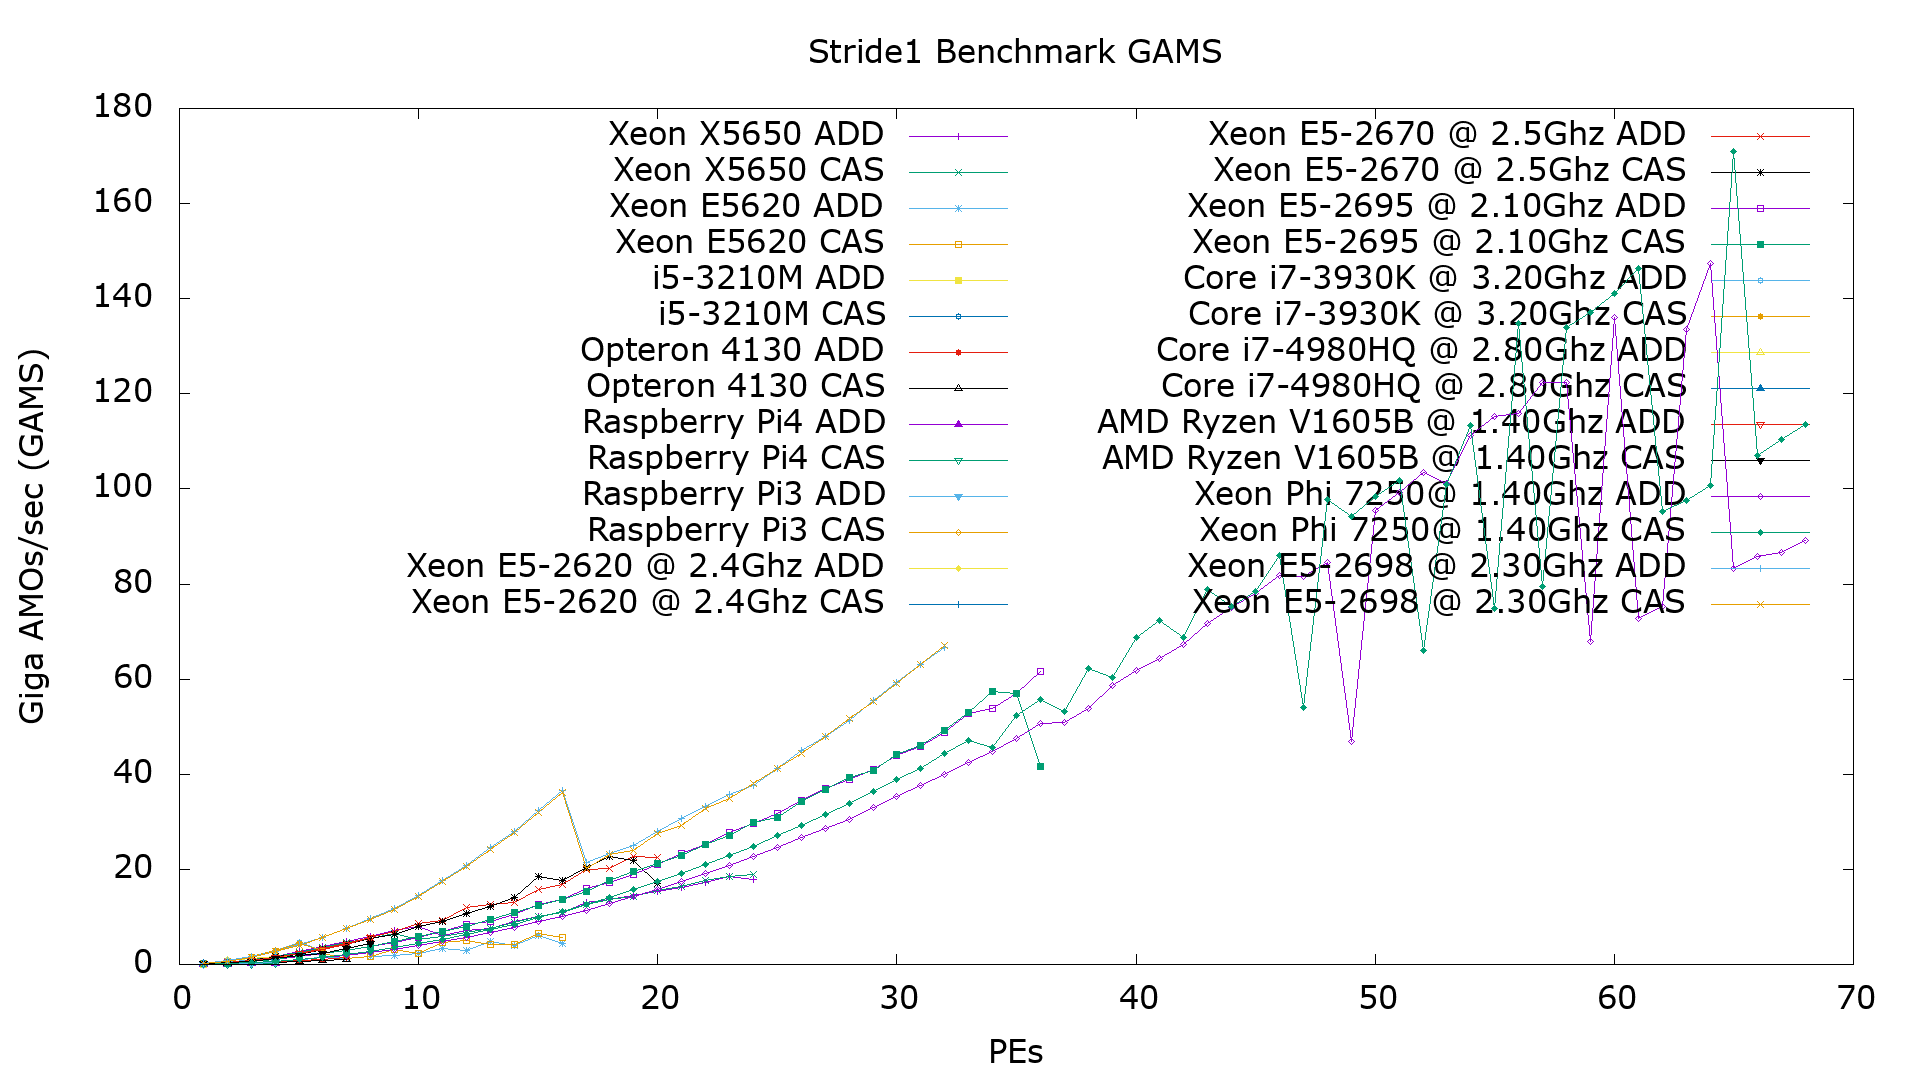
\includegraphics[width=3.5in]{figures/STRIDE1_GAMS.png}
\caption{Stride-1 Benchmark GAMS}
\label{fig:s1_gams}
\end{figure}

\begin{figure}[!t]
\centering
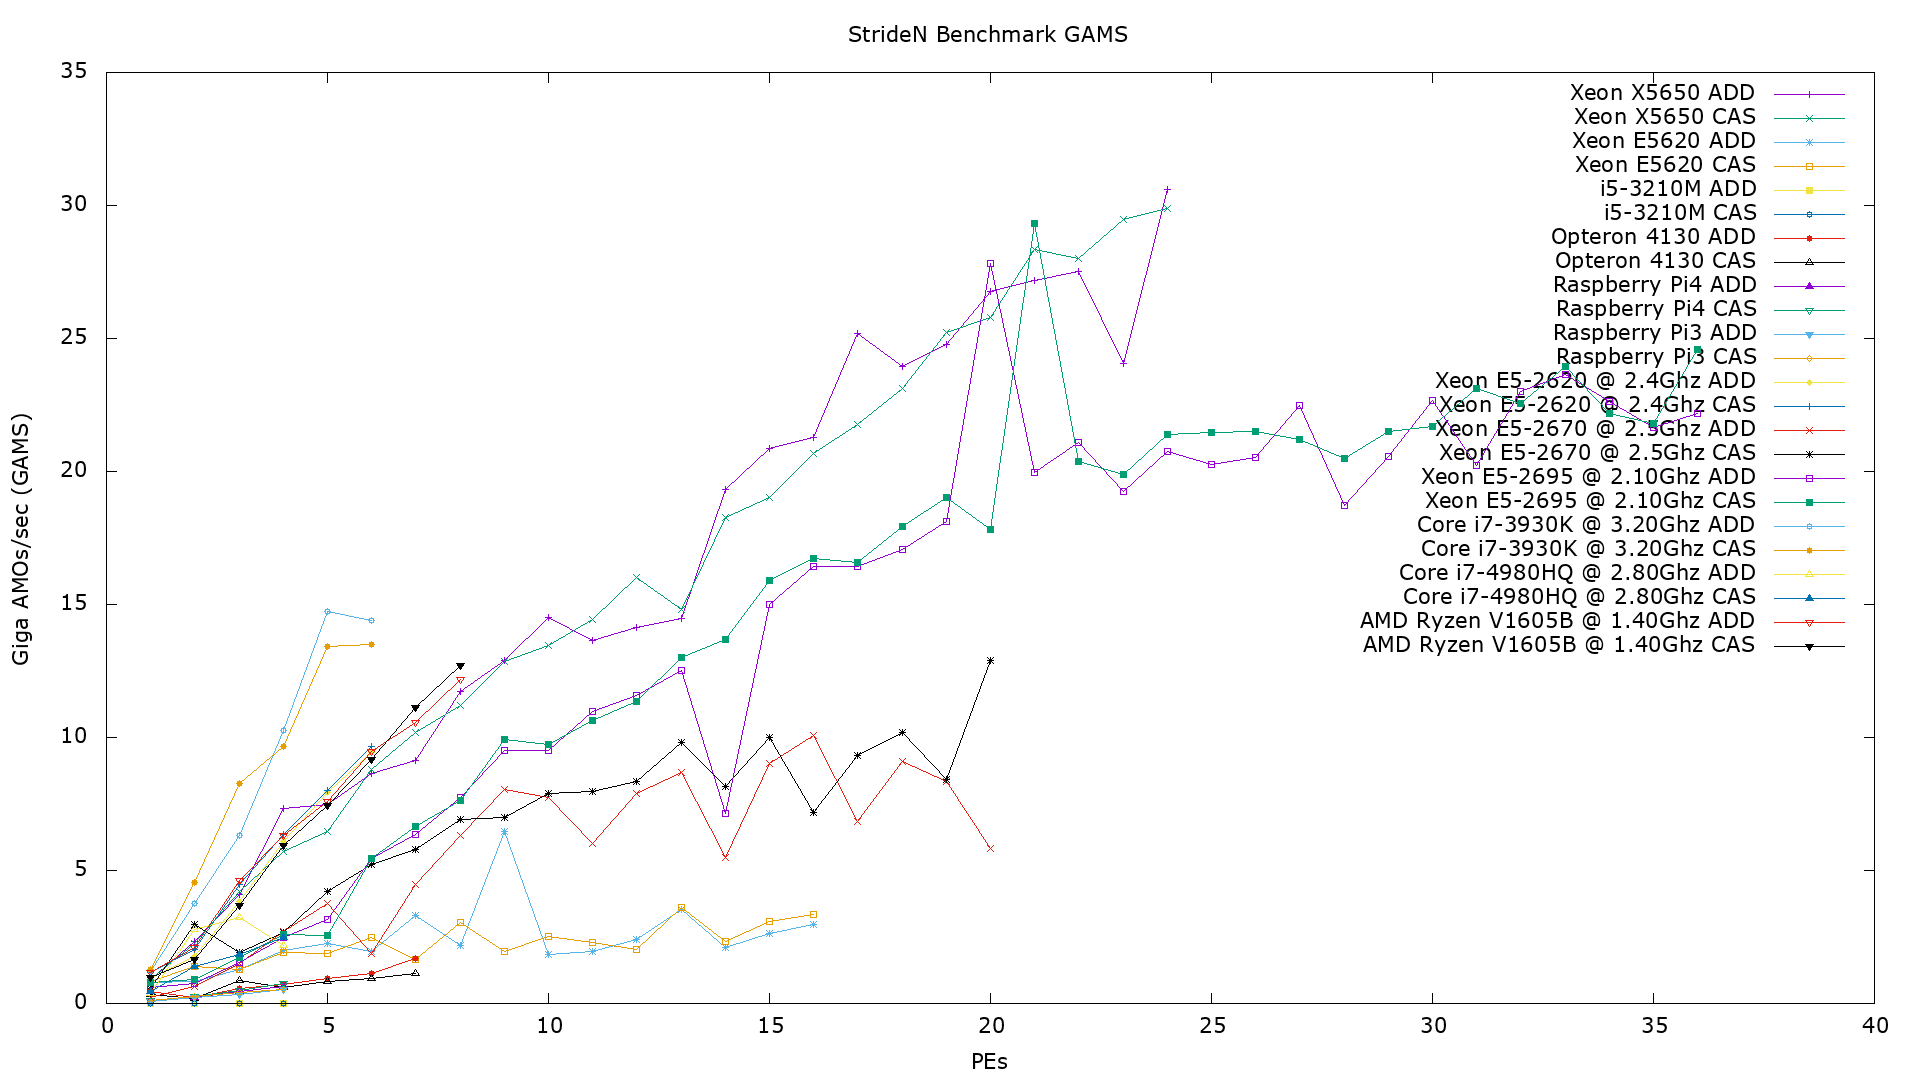
\includegraphics[width=3.5in]{figures/STRIDEN_GAMS.png}
\caption{Stride-N Benchmark GAMS}
\label{fig:sn_gams}
\end{figure}
